\section{Performance}

We test the performance of AVIST on a desktop computer, running Windows 7 Enterprise, which is equipped with an Intel i7 processor and a NVIDIA GeForce GTX 680 graphics card with 4GB memory. We use the network traffic dataset from case study one as our benchmark.  

\begin{figure}[htb]
	\centering
	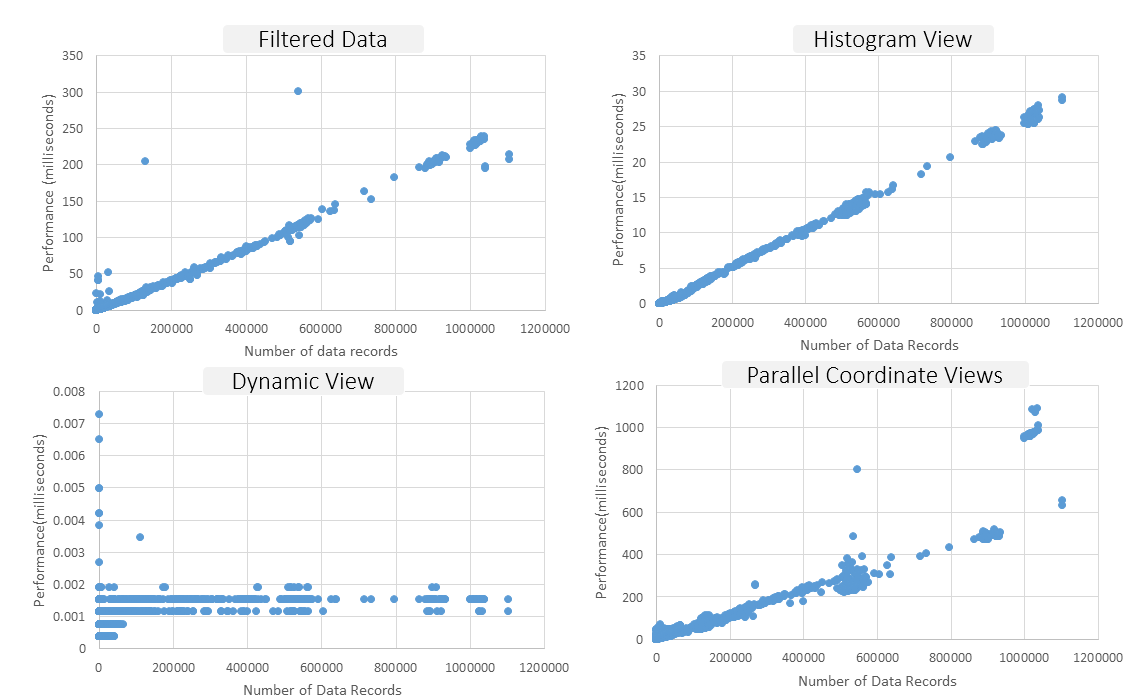
\includegraphics[width=1.0\linewidth]{pic/perf.png}
	\parbox[t]{1.0\columnwidth}{\relax
	}
	%
	\caption{\label{fig:performance}
		The performance of AVIST. The scatter plots show the relationship between number of queried data records and the performance (milliseconds). From the top left to the bottom right are the performances of filtered data, histogram view, time-series view and parallel coordinate views (four axes).  }
\end{figure}

We characterize  AVIST performance in two stages. The first stage is about filtered data generation, which is shared by all data views. The second stage is about each data view visual primitives generation, and their performance are independent with each other. Figure \ref{fig:performance} shows the tested performance in scatter plots. 
It shows a linear relationship between the performance and the queried data records beside time-series view.
Actually, the aggregated information in time-series view can be easily derived by the filtered dataset. The performance of parallel coordinate view is the bottleneck of AVIST. In the plot, we see that if the number of queried records exceeds 600,000, AVIST can not afford real time animation and interaction due to the hardware computation limitation. This also suggests that  users should filter more data in current time window or shrink the time window  for drilling down data details.

\begin{figure}[htb]
	\centering
	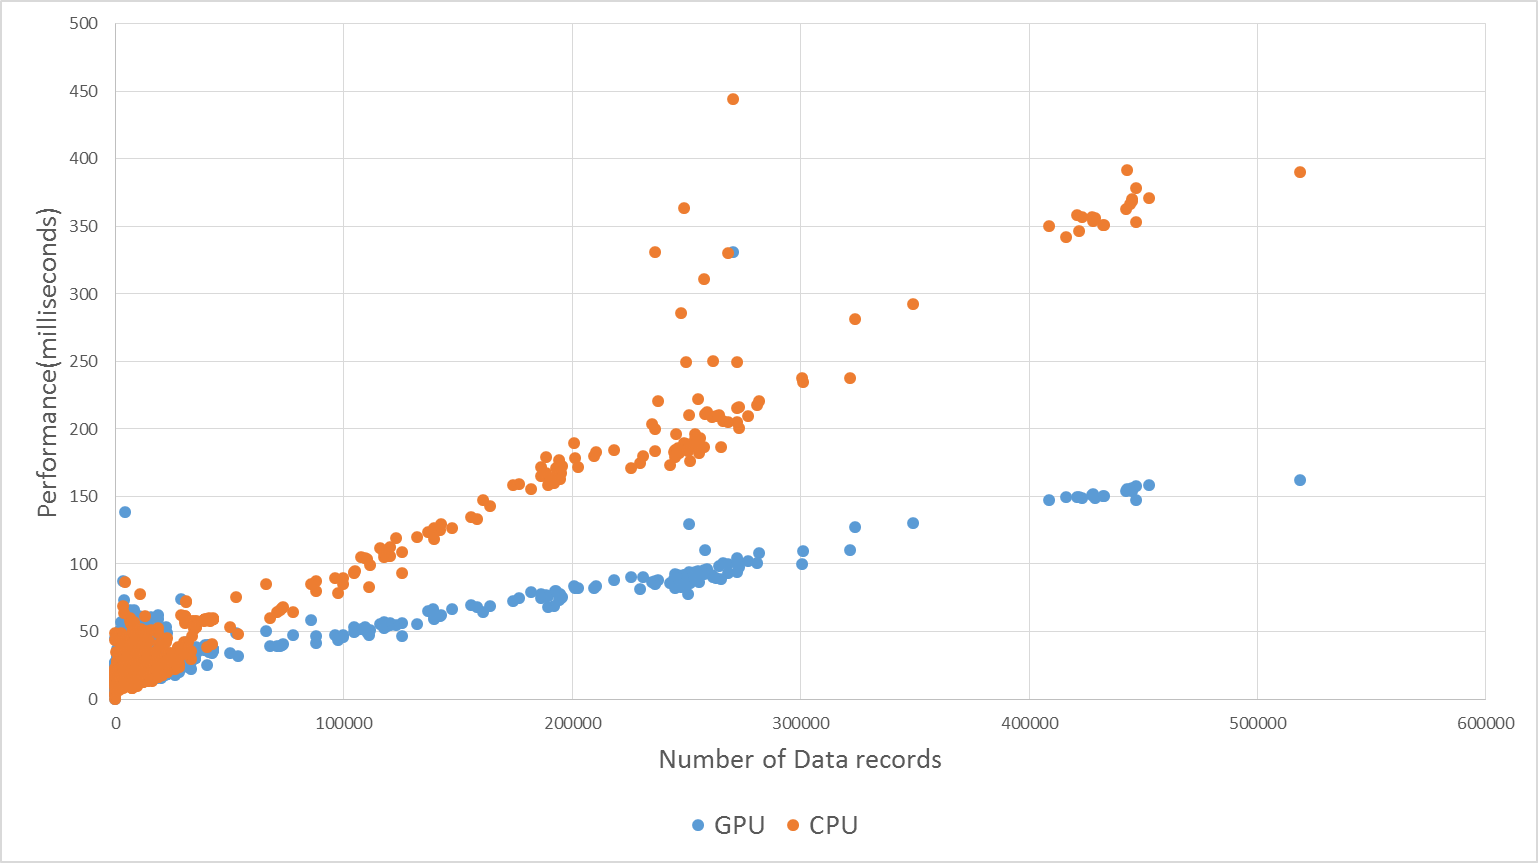
\includegraphics[width=0.75\linewidth]{pic/cmp.png}
	\parbox[t]{1.0\columnwidth}{\relax
	}
	%
	\caption{\label{fig:cmp} The performance comparison between CPU and GPU of parallel coordinate plots (two axes) }
\end{figure}

We also compare the performance between CPU and GPU. Figure~\ref{fig:cmp} shows the comparison of parallel coordinated plots generated by CPU and GPU. We see that the performance of CPU and GPU both follow the linear relationship with the number of data records. However, the performance of GPU is about 2.7 times faster than CPU.
